%Document Class
\documentclass[twocolappendix]{latex/emulateapj}

%Packages and Commands
%PACKAGES
\usepackage{multirow,color,wrapfig,ulem}
\usepackage {graphicx}
\usepackage{amsmath}
\usepackage[dvips]{epsfig}
\usepackage{fancyhdr}
\usepackage{epsfig}
\usepackage{graphicx}
\usepackage{amsmath}
\usepackage{amssymb}
\usepackage{latexsym}
\usepackage{epic}
\usepackage{hyperref}

%COMMANDS
\newcommand{\Msun}{{\ifmmode{{\rm {M_{\odot}}}}\else{${\rm{M_{\odot}}}$}\fi}}
\newcommand{\kms}{{\ifmmode{{\mathrm{\,km\ s}^{-1}}}\else{\,km~s$^{-1}$}\fi}}
\newcommand{\lya}{{Ly-$\alpha$~}}

\newcommand{\tauh}{{$\tau_{\rm H}$~}}
\newcommand{\vrot}{{$v_{\rm rot}$~}}
\newcommand{\vout}{{$v_{\rm out}$~}}

\newcommand{\ang}{{$\theta_{gal}$~}}
\newcommand{\lognh}{{$\log{n_H}$~}}
\newcommand{\nh}{{$n_H$~}}

\begin{document}

\title{Influence of galaxy rotation and outflows in the Lyman-$\alpha$
  spectral line}
\shorttitle{Rotation and outflows in the Lyman-$\alpha$ lines} 

\shortauthors{Remolina-Gutierrez and Forero-Romero.}

\author{Maria Camila Remolina-Gutierrez, Jaime E. Forero-Romero} 
\affil{Departamento de F\'{i}sica, Universidad de los Andes, Cra. 1
  No. 18A-10, Edificio Ip, Bogot\'a, Colombia} 
\email{mc.remolina197@uniandes.edu.co}
\email{je.forero@uniandes.edu.co}

\keywords{Galaxies: high-redshift, Lyman Alpha Emission, Galaxy
  Rotation, Galaxy Outflows, Radiative Transfer}   

\begin{abstract}
\noindent Young galaxies in the Universe have a strong \lya emission
caused by the ionized Hydrogen atoms in their interstellar
medium. When the spectrum of a galaxy has an intense peak around the
\lya natural frequency ($2.46\times 10^{15}$ Hz) it is called a Lyman
Alpha Emitter (LAE). Typical LAEs are very distant ($z \gtrsim
2$). This makes that all the data astronomers can obtain from them is
their spectra, and from there all the physical information of the
galaxy must be derived. Trying to solve this task requires the
creation of a simplified and solid model. In this paper we propose to
consider LAEs as a spherical distribution of Hydrogen atoms that
undergoes a solid body rotation and a radial expansion due to
outflows. We use radiative transfer Monte Carlo simulations to
interpret the Lyman-$\alpha$ line morphology. The main conclusion is
that this new model reproduces LAEs observed features in a clear way
and with consistent physical parameters. We also show results of
adjusting observational data for some selected objects to models with
and without bulk rotation. We finalize by discussing the possible
implications for these results in terms of the energetics required for
supernova feedback and outflows in high redshift galaxies. \\ 

REVISAR AL FINAL...\\
\end{abstract}

\section{Introduction}
\label{sec:intro}

Distant galaxies are key to understand early evolutionary stages of
our Universe.
However, those galaxies are challenging to detect.
Physical conditions in those galaxies allows the emergence of
Lyman-$\alpha$ line emission at $1216$ \AA \cite{PartrigePeebles}.
Galaxies detected through its Lyman-$\alpha$ emission receive the name of
spectra at  and named Lyman Alpha Emitters (LAEs).


In the early Universe the most abundant elements were Hydrogen(H) and
Helium(He), causing young galaxies to be rich in H atoms. Due to
stellar activity in a galaxy, the surrounding gas is ionized, so H
atoms excite and emit radiation at definite frequencies. The most
basic of these frequencies corresponds to the \lya line equal to $2.47
\times 10^{15}\;Hz$ \cite{PartridgePeebles}. This is equivalent to a
wavelength of 1215.67 $\AA$ cause by the transition of the H atom
electron from levels $2\rightarrow1$ dubbed Lyman Alpha ( \lya)
transition, discovered by Theodore Lyman in 1906. \cite{LymanBio} \\ 

Due to the amount of H atoms inside a galaxy, the whole body becomes a
strong \lya radiator. If the galaxy spectra shows a strong \lya line,
it classifies as a Lyman Alpha Emitter
(LAE). (\cite{DjorgovskiThompson}, \cite{Rhoads00},
\cite{Gawiser2007}, \cite{Koehler2007}, \cite{Ouchi08},
\cite{Yamada2012}, \cite{Schenker2012}, \cite{Kulas12},
\cite{Yamada2012}, \cite{Chonis2013}, \cite{Finkelstein2013},
\cite{Ostlin14}, \cite{Hayes2014}, \cite{Faisst2014},
\cite{Fumagalli2015}). However, when a \lya photon is emitted inside
the galaxy, it travels through its interstellar medium (ISM). During
the photon's path it can be absorbed and re-emitted by other H
atoms. The new frequency of the photon is different that the initial
one, in an observer frame of reference due to the atom's velocity. In
LAEs, the state of the ISM gas, before and after a photon's
re-emission is pretty much the same. This allows a random walk
approximation and lets us consider photon-atom encounters as
scatterings. A photon's scattering can happen several times and stops
only until the photon is able to escape the galaxy. \\ 

In a static galaxy, this random walk process produces a spectrum with
two equal and symmetric peaks around the natural \lya wavelength and
zero intensity at the center (Fig. A3 from \cite{CLARA}). If now the
gas has a bulk velocity, the shape of the \lya profile changes. We
explore these effects in this paper by proposing a new model for a
LAE. The model consists of a spherical distribution of H atoms
undergoing a solid body rotation and radial expansion (outflows). \\ 

Our main goal with this work is to measure the effect of the model's
physical parameters on the outgoing \lya line. In this case, due to
the resonant\footnote{Resonant is a common term used in radiative
  transfer. It means that the photons that create the line are
  absorbed and re-emitted several times before escaping the cloud of
  gas.} nature of the \lya line, analytical solutions can not be
derived. Because of this, it becomes necessary to run simulations that
explore and test the model. In this paper we use the radiative
transfer code \textbf{CLARA} (Code for Lyman Alpha Radiation Analysis)
written by Forero-Romero et al. \cite{CLARA}. CLARA can simulate the
\lya line of a spherical rotating LAE depending on its mass and
velocity, so we modify it to include outflows and then we explore the
resulting consequences on the \lya line. \\


 

\section{A new LAE model}
\label{sec:newmodel}

We model spherical galaxy to facilitate the interpretation of the results, by deleting what would be another degree of freedom regarding a different geometry. Furthermore, this approximation is commonly used in the literature, as it explains a wide variety of observational features (\cite{Ahn03}, \cite{Verhamme06}, \cite{Dijkstra06}). \\

There are 3 parameters in this model that define a LAE: the rotational velocity (\vrot), the outflow velocity (\vout) and the optical depth (\tauh). \vout is due to material ejected from the galaxy, by supernovas(\cite{Verhamme06}, \cite{Orsi12}, \cite{Hashimoto2015}, \cite{Gronke2015}). \tauh roughly corresponds to number of H atoms found by a \lya photon if one traces a line from the center of the galaxy to its edge, and it resembles the mass of the LAE.\\

In this model, the LAE has a bulk velocity corresponding to the superposition of rotation and outflows, as shown in Fig. \ref{fig:model}. The velocity components are written in Eqs. (\ref{eq:vx}) (\ref{eq:vy}) (\ref{eq:vz}). In these equations, $R$ is the radius of the sphere; $x$, $y$ and $z$ are the coordinates in a cartesian frame; and the $\mp$ signs in $v_x$ and $v_y$ indicate the direction of rotation, respectively. This rotation is a solid body rotation and its direction goes according to the right hand rule applied to the $\hat{k}$ unit vector. The outflow velocity is dependent on the position relative to the center of the galaxy, being it zero at the center and maximum at the edge of the sphere.\\

\begin{equation}
	v_{x}=\frac{x}{R}v_{\rm out}-\frac{y}{R}v_{\rm rot} 
	\label{eq:vx}
\end{equation}

\begin{equation}
	v_{y}=\frac{y}{R}v_{\rm out}+\frac{x}{R}v_{\rm rot} 
	\label{eq:vy}
\end{equation}

\begin{equation}
	v_{z}=\frac{z}{R}v_{\rm out}
	\label{eq:vz}
\end{equation}

These 3 parameters, \vrot, \vout and \tauh, leave the idea of a model of LAE, that although simple, considers the main galaxy's dynamics. All of them have been previously proposed and used by different authors, but never combined together (\cite{Adams72}, \cite{Harrington73}, \cite{Neufeld90}, \cite{Dijkstra06}, \cite{Verhamme06}, \cite{Forero12}, \cite{Martin2015}, \cite{Garavito14}, \cite{Neufeld91}, \cite{Laursen09}, \cite{Barnes11}, \cite{Verhamme12}, \cite{Yajima12}).\\

%mirar donde pongo esto
However, in the plots shown in this paper we use instead velocity, $V$, units. This eases the comparison against observational data. The velocity units are defined by
The units of $V$ are usually \kms. In this case, the photon is redshifted in frequency when the velocity is greater than 0, and blueshifted in the opposite case. \\

The initial emission of photons is taken at the center of the sphere for practicality due to the fact that both, center and off-center emissions, give analogous results. From here, $100000$ photons are emitted with the natural \lya wavelength and start to scatter. When each photon is re-emitted, its new wavelength depends on the H atom's velocity (both thermal and bulk) and direction (both initial and final). However the photon's new direction of propagation is random in the rest frame of the atom. \\ 

The individual scattering of all the photons is tracked through the complete 3D Hydrogen distribution. Once each photon escapes the galaxy, its final values are stored: position $\vec{r}$, direction of propagation $\hat{k}$, dimensionless frequency $x$, and number of scatterings $N$. To build the observed spectrum we make a histogram of the escape frequencies $x$. The number of scatterings $N$ tells how many steps the random walk requires to reach a distance to the center that is $\geq R$. In order to avoid situations in which the photon has not escaped after a long computational time, CLARA defines a number $N_{max}$ so the code stops. However, according to statistics, this last situation has low probabilities, so the photon is always most likely to exit the sphere. \\

%The process that takes place from the moment the first photon is emitted to the moment the last photon escapes the sphere, is called a simulation. Each simulation runs in the scientific computational cluster of Universidad de los Andes due to the computing resources it requires. Depending on \tauh, we need a different number of processors in order to minimize the time demands. For \tauh $=10^5, 10^6, 10^7$ we use 6, 12, 24 processors, respectively. The running times go from 7 hours to 1 week approximately, depending on the case. \\

\subsection{Galaxy's Viewing Angle}
An observer located far away, only receives photons emitted along its line of sight. That means, only photons escaping in the direction of the observer must be counted in the spectrum. In the simulation we approximate this by taking into account only the photons with escaping direction angle $\theta$ respect to the rotation axis within the range $[\theta_{min}-\theta_{max}]$. We illustrate this in Fig. \ref{fig:model}. \\

\begin{figure}[h!]
	\begin{center}
		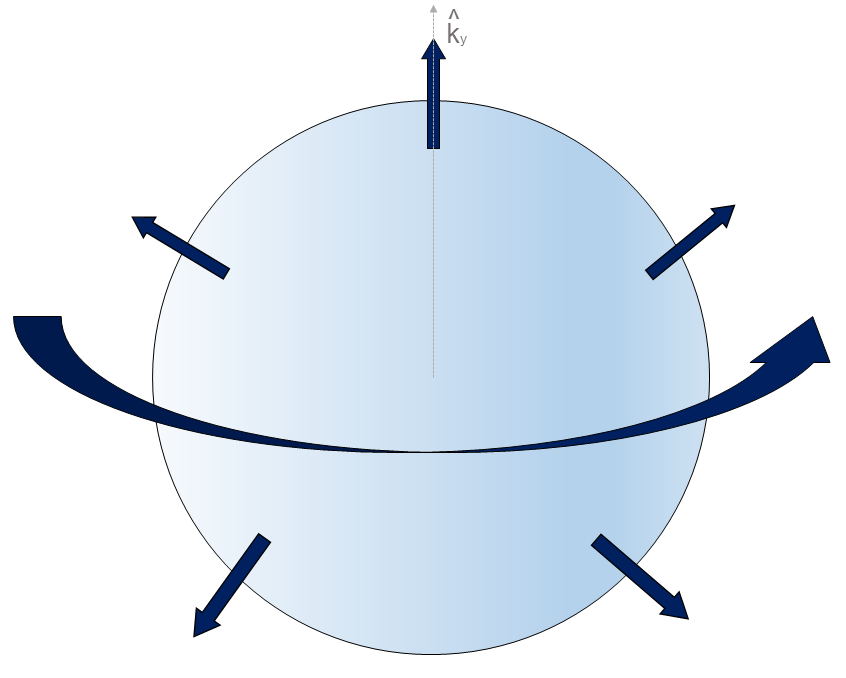
\includegraphics[width=0.48\textwidth]{./figures/model}
	\end{center}
	\caption{\textbf{Model:} Spherical LAE with tangential and radial velocities due to rotation and outflows, respectively. The galaxy cut is in the $y-z$ plane perspective. The observer is located at an specific viewing angle of the sphere. Only photons with a direction that enters in this range of vision are taken into account to build the observed spectrum.
		\label{fig:model}}
\end{figure}

Therefore, in principle the spectra depend on two new parameters, the azimuthal and the polar angle. However, the galaxy's motion is symmetrical respect to its rotation axis. This implies that the resulting spectrum is independent from the azimuthal angle. Taking into account this symmetry, we only select photons on their polar angle, regardless of their azimuthal angle. Regarding the polar angle, we build the spectra for observers located on 3 different positions, with $\theta$ intervals uniformly distributed in $\cos(\theta)$. \\ 

To summarize, the parameters influencing the spectra are \vrot, \vout, \tauh and $\theta$. In the next section we evaluate the impact each of these has on the resulting profile. \\


\section{Results}
\label{sec:results}

\subsection{Resulting simulated spectra}
In order to define the ranges of \tauh, \vrot and \vout, it is necessary to refer to observational constraints. The common values for typical LAEs that were set as parameters are in Tab. \ref{tab:values}. We run CLARA's modified version for all the permutations of these 3 parameters. \\

\begin{table}[htbp]
	\centering
	\begin{tabular}{|c|c|c|}
		\hline
		$\tau_{\mathrm{H}}$ & $v_{rot}$ (\kms) & $v_{out}$ (\kms) \\
		\hline
		$10^5$, $10^6$, $10^7$ & 50, 100 & 5, 10, 15, 20, 25, 50, 75 \\
		\hline
	\end{tabular}
	\caption{\textbf{Parameters' Values:} All consistent with a LAE's typical properties}
	\label{tab:values}
\end{table}

The behavior of the resulting sets of spectra can be summarized by Fig. \ref{fig:summary}. We concluded from the simulations a clear creation of two asymmetric peaks around $V=0$ \kms with the tallest peak always redshifted. We detected a strong dependence on the outflow velocity that induces the peak asymmetry. We also detected that the rotation velocity broadens the line horizontally. Both these effects have been previously reported separately in the literature, so these results can valid their superposition to some extend. \\

\begin{figure}[h!]
	\begin{center}
		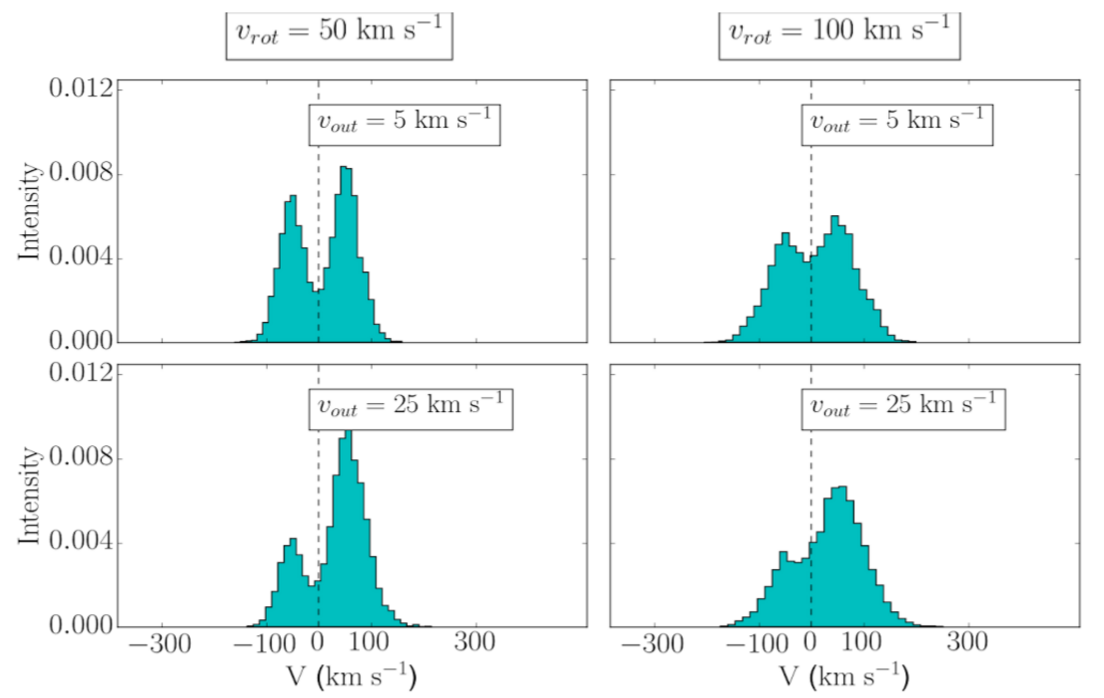
\includegraphics[width=0.48\textwidth]{./figures/summary}
	\end{center}
	\caption{\textbf{4 different \lya profiles:} With \tauh$=10^5$ and $\theta \simeq 90^\circ$. The rotational velocity \vrot increases to the right and the outflows velocity \vout increases downwards. The intensity is in arbitrary units.
		\label{fig:summary}}
\end{figure}

\subsection{Influence of the viewing angle $\theta$}
We take now into account the viewing angle of the galaxy to build the observed spectra. For all of the physical parameters' combinations, the effect of $\theta$ in the \lya line is always the same.\\

\begin{figure}[h!]
	\begin{center}
		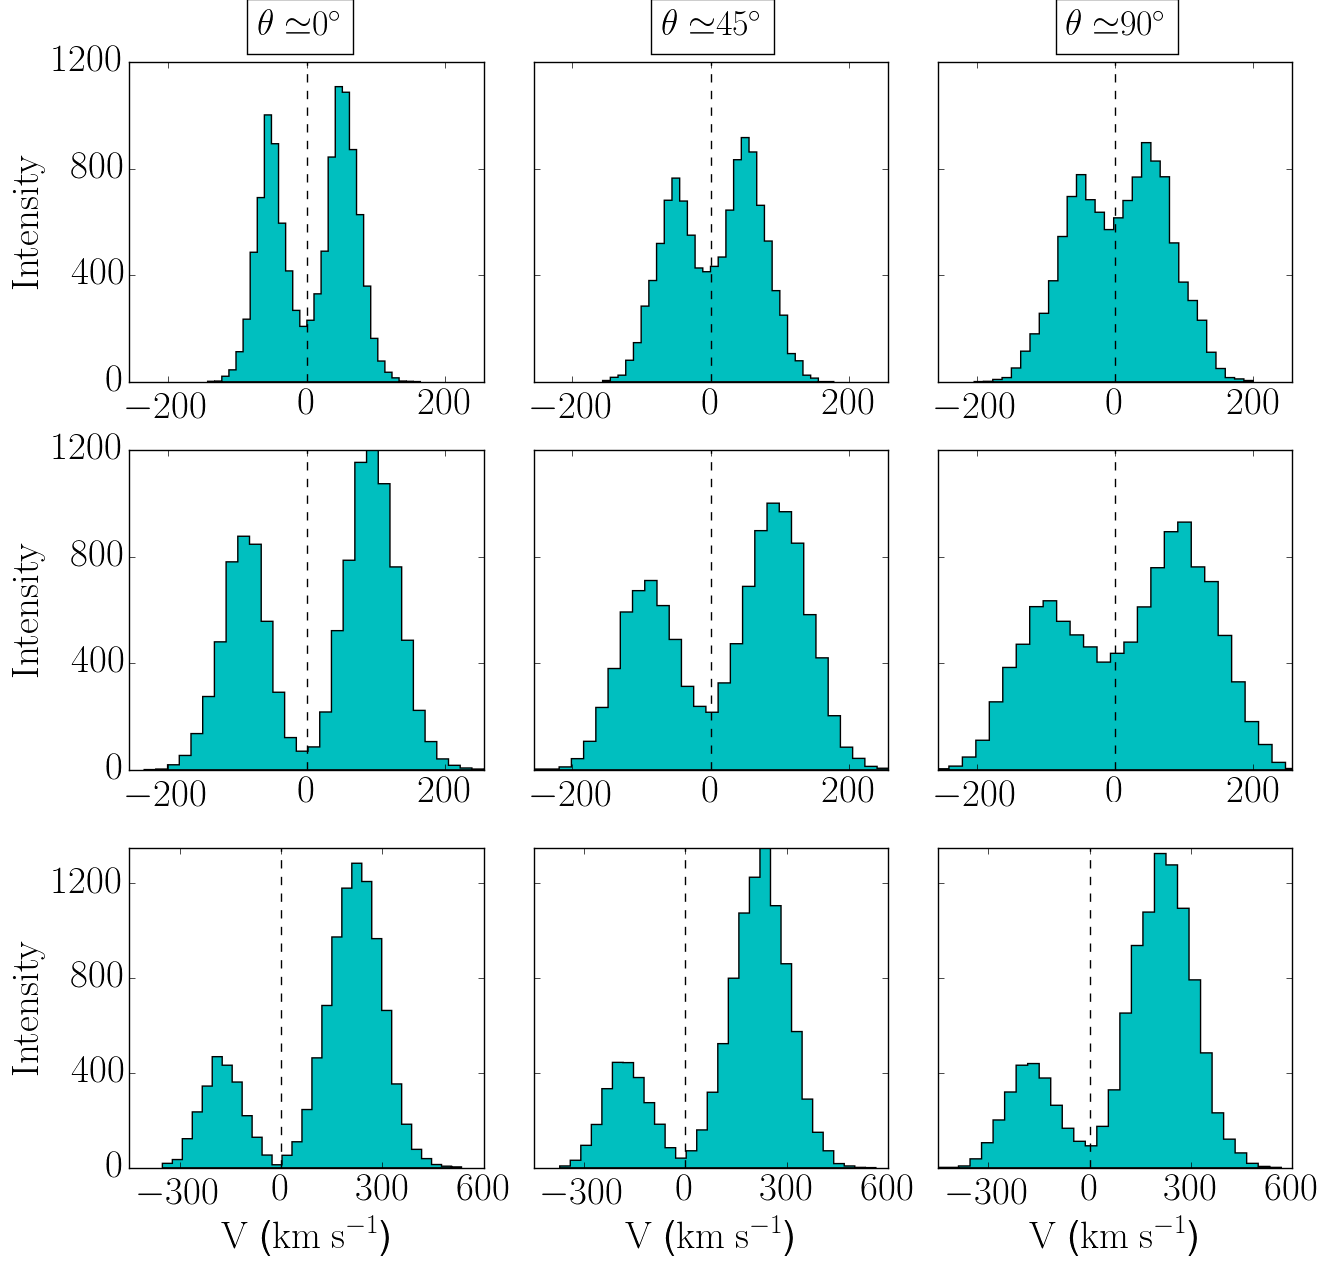
\includegraphics[width=0.5\textwidth]{./figures/angles}
	\end{center}
	\caption{\textbf{\lya profile for different $\theta$.} For \tauh$=10^5$, \vrot$=50$ \kms and \vout$=20$ \kms. For \tauh$=10^6$, \vrot$=100$ \kms and \vout$=5$ \kms. For \tauh$=10^7$, \vrot$=100$ \kms and \vout$=15$ \kms. The intensity is in arbitrary units.
		\label{fig:angles}}
\end{figure}

From Fig. \ref{fig:angles} it is clear that the intensity of the valley between the two peaks increases along with $\theta$. This causes an intensity decrease in the rest of the frequencies, thus a broadening of the line. The asymmetry also changes with the viewing angle.\\


\subsection{Morphology of \lya line}

To summarize, the influence of the 4 parameters on the \lya morphology is the following: 

\begin{itemize}
	\item \tauh induces a redshift. Increasing the optical depth separates the line of the zero velocity line. \\
	\item \vout decreases the right peak's intensity. Higher \vout makes the left peak smaller until it merges with the right one. \\
	\item \vrot broadens the line and decreases the maximum intensity. Higher \vrot implies a flatter spectrum. This effect has not been deeply studied in literature. Only Garavito et al. \cite{Garavito14} has simulated its effect. Our results are consistent with their conclusions.
	\item $\theta$ increases the central valley of the line. Higher $\theta$ makes more emission at \lya natural frequency. \\ 
\end{itemize}

\subsection{Doppler shift by rotation}

The rotation effect induces a Doppler shift in frequency and displaces the only-outflow spectra. As seen in Fig. \ref{fig:rotation_doppler_outflow} rotation takes the resulting spectrum with \vrot$=0$ and displaces it from its central location. Then it weights the lines and they all merge into the resulting red \lya line.\\

\begin{figure}[h!]
	\begin{center}
		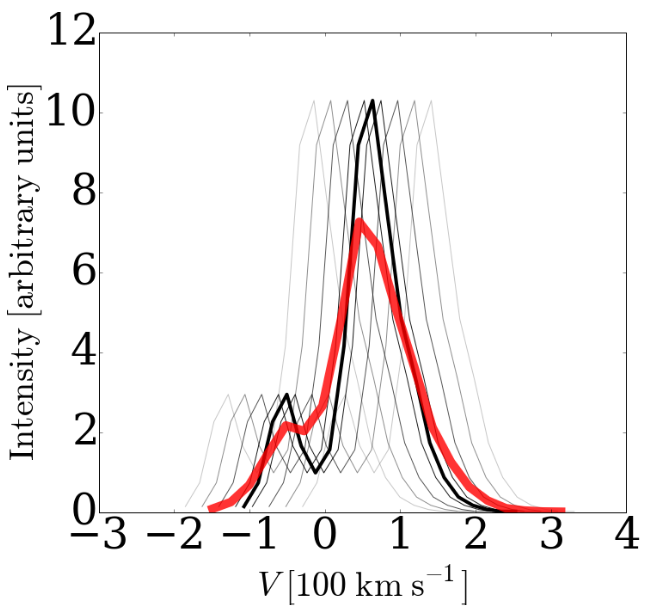
\includegraphics[width=0.3\textwidth]{./figures/rotation_doppler_outflow}
	\end{center}
	\caption{\textbf{Rotations induces a Doppler shift of the only-outflow spectra:} Each of the black lines is then weighted to obtain the red line.
		\label{fig:rotation_doppler_outflow}}
\end{figure}

PONER GRAFICA REAL...\\

\section{Observational Implications}
\label{sec:observationalimplications}

Among the observational implications that this paper has over observations we select three principal ones. First, the rotational effects of the galaxy should be clearly detected and characterized by MUSE's high resolution data. The Doppler redshift is already visible in other observations, such as the one seen in Fig. 7 of Prescott et al. \cite{Prescott14}.\\

Second, the central ($V=0$) emission of the spectra seen in the results is a consequence of the viewing angle of the galaxy and can be controlled by it. This means that the reason is not necessary that radiation is escaping without scattering, as several authors have suggested (CITAS...).\\

Finally, all the spectra produced from this new LAE model is roughly consistent with observations. The consideration of adding the new rotation parameter to the standard only-outflow model found in literature is reasonable and very powerful. \vrot and its consequent viewing angle $\theta$ can modify the morphology of the \lya line in new different ways by keeping the model simplified.\\

\section{Conclusions}
\label{sec:conclusions}

In this paper, the objective was to analyze and measure the influence of galaxy rotation and outflows on the \lya line. The motivation for this is to be able to obtain physical information of a LAE by just looking at its \lya profile. In order to accomplish this objective, we propose a new model of a LAE consisting of a sphere of Hydrogen atoms that expands radially and rotates as a solid body. A modified version of the program CLARA \cite{CLARA} is used to set the conditions and emulate the radiative transfer process inside the galaxy. \\

The conclusions obtained from this work are: 

\begin{itemize}
	\item The outgoing spectra depend on the angle an external observer is viewing the galaxy from. The closer it is to the equator of the galaxy, the higher the central valley of the frequency distribution. 
	
	\item The effects of \vrot, \vout and \tauh are consistent with the different authors that have used them. \vrot broadens the \lya line. \vout increases the peaks asymmetry and \tauh induces a redshift around the zero velocity.
	
	\item Rotations induces a Doppler shift in frequency of the only-outflow spectra.
	
	\item The final spectra obtained are roughly consistent with LAEs observations. \\ 

\end{itemize}

\subsection{Future work}

For future work regarding the model, we would like to implement a differential rotation for the LAE instead of solid body. Regarding result analysis, we would like to compare against observations in two ways. Firstly by using the kinematic observation obtained from newly observed LAEs. We could do a consistency check between their real spectra and the simulated one that our model would produce with the respective parameters. Secondly we would like to take a specific observed spectrum and fit it using MCMC in order to predict ranges for its parameters. \\

\subsection{Reproducibility}

All of this work is available online and free to use to anyone. The data, source code and instructions to replicate this paper's results are in the GitHub repository:  \texttt{github.com/astroandes/CLARA\_RotationOutflows}. \\


\section*{Acknowledgments}
The authors would like to acknowledge the high performance computational cluster (HPC) hosted by Universidad de los Andes, where we ran the simulations for CLARA. \\

We would also like to acknowledge the participants of the meeting \textit{Escape of Lyman radiation from galactic labyrinths} at Crete, Greece, for their valuable comments on this work, specially to Max Gronke and Christian Herenz. \\


%------------------------REFERENCES----------------------------

\bibliographystyle{latex/apj}
\bibliography{references}

\end{document}
